%
% do not add anything in this part
%
\ifx\onefile\undefined

	\documentclass{article}

	%if tcolorbox and tikz are installed use next line
	%\usepackage[tcbox]{projectalgo}
	\usepackage{projectalgo}

	% replace type by one of graph, math, combinatory, string, network, datastructure, ai, image
	\pbtype{type}

	\begin{document}
\fi

%
% things can be added below
%

\def\pbname{Fast/Disrete Fourier Transform} %change this, do not use any number, just the name

\section{\pbname} 

% only for overview, so short description (no more than 1-2 lines)
\begin{overview}
\item [Algorithm:]Cooley-Tukey algorithm~(algo.~\ref{problem39}) 
	% - replace nb with problem number (e.g. problem101)
	% -	must match the label of the algorithm 
	% - for more than one algo list each of them and use problem101a, problem101b, problem101c etc.
\item [Input:] A finite sequence $f$ of length $n$ which is a equally-spaced sample of a function.
\item [Complexity:]  $\mathcal{O}(n\log{n})$
\item [Data structure compatibility:] N/A
\item [Common applications:] Spectral Analysis, data compression, filter bank, solving partial differential equations, etc.
\end{overview}



\begin{problem}{\pbname}
	Converting a finite sequence of equally-spaced samples of a function in the original domain into a same-length sequence of equally-spaced samples in the frequency domain
\end{problem}

\subsection*{Description}
Fourier transform is a way to convert a function in its original domain (usually time domain) into frequency domain. The main strategy is to see functions as an accumulation of sine waves in different frequency, which can also be denoted that as $$f(x) = \int_{-\infty}^{\infty}F(s)e^{2i\pi sx} ds$$

in which $F(s) = \int_{-\infty}^{\infty}f(x)e^{-2i\pi sx} dx$. 

The formula is written in the exponential way to express sine functions, where the functions of $s$ and $-s$ will be combined into a sine wave. By Fourier transform the ditribution of the function in different domains can be found easily, thus spectral analysis and some signal processing diveces such as filters can be implemented more easily. This can also be used in Mathematics to analyze the behaviour of a function or in solving differential equations.

However, since computers does not have the ability to store continuous data in the memory and it also cannot generate a continuous sequence of data which represents the frequency-domain function, a new method sohuld be used such that the implementation only concerns with discrete time data which computers can collect and generate, and that is why discrete fourier transform is introduced. Discrete Fourier transform requires a finite sequence $f$ as an input, which indicates a equally-spaced sample of data of the function. The output of discrete fourier transform is also a sequence $F$ which also represent a sample of data in the frequency domain. The formula is given below.

\begin{align*}
    F[k] &= \sum_{x=0}^{n-1}f[x]\cdot e^{-2ki\pi x/n}dx\\
    &=\sum_{x=0}^{n-1}f[x]\cdot[cos(2\pi kx/n)-i\cdot sin(2\pi kx/n)]
\end{align*}

From the given formula, we can see that if brute force is applied to calculate discrete fourier transform, calculating a certain value in $F$ needs an $\mathcal{O}(n)$ complexity to add up all terms. And since there are $n$ elements in $F$, the brute force algorithm is of $\mathcal{O}(n^2)$ time complexity.

And actually this algorithm can be optimized, and so fast fourier transform is introduced. The optimizing way is based on the idea of divide and conquer. If the Fourier transform of two halves of the sequence is generated, then due to some mathematical basis, the Fourier transform of the whole sequence can be deduced more easily.

Here one of the methods called Cooley-Tukey algorithm will be discussed and for convenience, let $n$ be a power of $2$ so that it can be easily be broken int o halves repeatedly. The state diagram of the algorithm is shown below, taking $n=8$ as an example:

\begin{figure}[h]
    \centering
    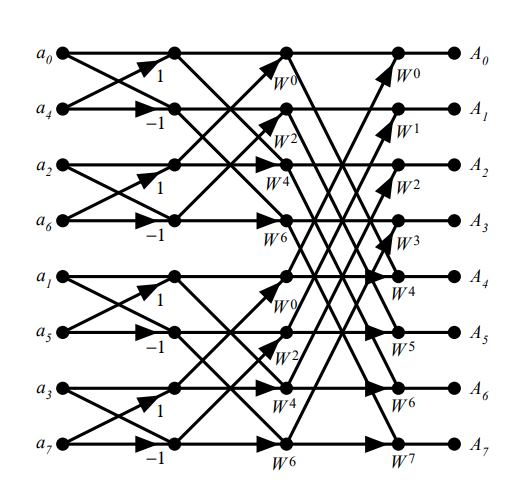
\includegraphics[scale=0.5]{problem38_1.png}
\end{figure}

Those $a_i$ on the left are the input and $A_i$ on the right are output. It can be seen that the inputs are not aligned in original order. In fact they are ordered in bit-reverse incrementing order, which will make the diagram more clear.

It also can be seen that each node in the middle part has two edges on the left which points two it. It means a weighted addition with respect to the value on the tip of the arrow. For example, the value of the second node in the second stage is $a_0-a_4$. The value $W$ in the latter stages is the value $e^{-2i\pi/n}$, and here it is $e^{-2i\pi/8}=(1-i)/\sqrt{2}$. In the $k_{th}$ last stage, the order of $W$ will increment by $2^{k-1}$ along the nodes and the modulo of $n$ will be taken. Of course in the first stage the order will be incrementing by $n/2$, then the number should be $1,-1,1,-1,...$. In this way, the discrete Fourier transform can be derived. 

Because for each stage, there will be $n$ numbers to be calculated, which costs $\mathcal{O}(n)$ complexity, and there should be totally $log_2{n}$ stages in total, so the total complexity is $\mathcal{O}(n\log{n})$

\newpage
% add comment in the pseudocode: \cmt{comment}
% define a function name: \SetKwFunction{shortname}{Name of the function}
% use the defined function: \shortname{$variables$}
% use the keyword ``function'': \Fn{function name}, e.g. \Fn{\shortname{$var$}}
\begin{Algorithm}[Cooley-Tukey Algorithm\label{problem39}]
	% - replace nb with problem number (e.g. problem101)
	% -	must match the reference in the overview
	% - when writing more than one algo use problem101a, problem101b, problem101c etc.
	\Input{A sequence $f$ with $n$ elements}
	\Output{The discrete Fourier transform of $f$}
	%	\Fn{\myfunction{$a,b$}}{
	%	}
	\For {$i\leftarrow 0 \text{ to }n-1$}{
        \uIf {$i<bit\_reverse(i)$}{
            swap($f[i],f[bit\_reverse(i)]$)\;
        }
    }

    
    W $\leftarrow e^{-2i\pi /N}$\;
    \For {$k\leftarrow 1 \text{ to }log_2n$}{
        b $\leftarrow$ a sequence of length $n$;
        
        w $\leftarrow W^{n/2^k}$\;
        \For {$m\leftarrow 0\text{ to }n-1$}{
            \uIf {$mod(m,2^k)<2^{k-1}$}{
                $b[m] \leftarrow f[m]+w^mf[m+2^{k-1}]$\;
            }
            \Else{
                $b[m] \leftarrow f[m-2^{k-1}]+w^mf[m]$\;
            }
            $f\leftarrow b$\;
        }
    }
    \Ret f\;
	

\end{Algorithm}

\subsection*{References}
% list references where to find information on the given problem
% prefer books, research articles, or internet sources that are likely to remain available over time
% as much as possible offer several options, including at least one which provide a detailed study of the problem
% if available include links to programs/code solving the problem

\begin{itemize}\itemsep .125cm
	\item \url{https://www.cs.cmu.edu/afs/andrew/scs/cs/15-463/2001/pub/www/notes/fourier/fourier.pdf}
	\item James W. Cooley, Peter A. W. Lewis, and Peter W. Welch, "Historical notes on the fast Fourier transform"
	\item \url{https://en.wikipedia.org/wiki/Fast_Fourier_transform}
\end{itemize}

\ifx\onefile\undefined
	\end{document}
\fi
